\documentclass[12pt, oneside, openany, titlepage]{article}

\usepackage{booktabs}
\usepackage{tabularx}
\usepackage{hyperref}
\usepackage{pdflscape}
\usepackage{graphicx}
\usepackage[normalem]{ulem}
\hypersetup{
    colorlinks,
    citecolor=black,
    filecolor=black,
    linkcolor=red,
    urlcolor=blue
}
\usepackage{xcolor}
\usepackage[round]{natbib}

%% Comments

\usepackage{color}

\newif\ifcomments\commentstrue %displays comments
%\newif\ifcomments\commentsfalse %so that comments do not display

\ifcomments
\newcommand{\authornote}[3]{\textcolor{#1}{[#3 ---#2]}}
\newcommand{\todo}[1]{\textcolor{red}{[TODO: #1]}}
\else
\newcommand{\authornote}[3]{}
\newcommand{\todo}[1]{}
\fi

\newcommand{\wss}[1]{\authornote{blue}{SS}{#1}} 
\newcommand{\plt}[1]{\authornote{magenta}{TPLT}{#1}} %For explanation of the template
\newcommand{\an}[1]{\authornote{cyan}{Author}{#1}}

%% Common Parts

\newcommand{\progname}{ProgName} % PUT YOUR PROGRAM NAME HERE
\newcommand{\authname}{Team \#, Team Name
\\ Student 1 name
\\ Student 2 name
\\ Student 3 name
\\ Student 4 name} % AUTHOR NAMES                  

\usepackage{hyperref}
    \hypersetup{colorlinks=true, linkcolor=blue, citecolor=blue, filecolor=blue,
                urlcolor=blue, unicode=false}
    \urlstyle{same}
                                


\begin{document}

\title{Verification and Validation Report: HairEsthetics} 
\author{Team 18 \\ Charlotte Cheng
        \\ Marlon Liu
        \\ Senni Tan
        \\ Qiushi Xu
        \\ Hongwei Niu
        \\ Bill Song}
\date{\today}
	
\maketitle

\pagenumbering{roman}

\section{Revision History}

\begin{tabularx}{\textwidth}{p{3cm}p{2cm}X}
\toprule {\bf Date} & {\bf Version} & {\bf Notes}\\
\midrule
Mar 6 & 1.0 & Upload Template\\
Mar 8 & 1.1 & Initial Draft\\
\textcolor{red}{Apr 3} & \textcolor{red}{2.0} & \textcolor{red}{Revision 1}\\
\bottomrule
\end{tabularx}

~\newpage

\section{Symbols, Abbreviations and Acronyms}

\renewcommand{\arraystretch}{1.2}
\begin{tabular}{l l} 
  \toprule		
  \textbf{symbol} & \textbf{description}\\
  \midrule 
  T & Test\\
  SRS & Software Requirements Specification\\
  HA & Hazards Analysis\\
  MG & Module Guide\\
  VnV Plan & Verfication and Validation Plan \\
  \bottomrule
\end{tabular}\\

\newpage

\tableofcontents

\listoftables %if appropriate

\listoffigures %if appropriate

\newpage

\pagenumbering{arabic}

\section{Functional Requirements Evaluation}

  \begin{tabular}{|p{2cm}| p{3cm}| p{3cm}| p{3cm}|p{2cm}| p{1cm}| }
    \hline
    TestID & Initial State & Input & Expected Results & Actual Results & Result \\ 
    \hline
    FRS-T1 & Home Page & A photo of a person's face uploaded by the tester with the upload button clicked & The facial features coordinates in a tuple (x,y), where x and y values are appropriate for the location of the facial features within the image & (-5, 2), indicating that the facial features were detected to be slightly left of center and slightly above the center of the image. & pass \\ 
    \hline
\end{tabular}


\begin{tabular}{ |p{2cm}| p{3cm}| p{3cm}| p{3cm}|p{2cm}| p{1cm}|} 
 \hline
 TestID & Initial State & Input & Expected Results & Actual Results & Result \\ 
 \hline
 HS-T1 & Home Page & A photo of a person's face uploaded by the tester with the upload button clicked & The facial features coordinates in a tuple (x,y), where x and y values are appropriate for the location of the facial features within the image & (-5, 2), indicating that the facial features were detected to be slightly left of center and slightly above the center of the image. & pass \\ 
 \hline

 HS-T2 & \Home Screen & \sout{A photo of a person's face taken by the tester through the camera in the web app}\textcolor{red}{User click on deny when asked for camera permission} & \sout{The facial features coordinates in a tuple (x,y), where x and y values are appropriate for the location of the facial features within the image}\textcolor{red}{Hairstyle disabled and error message should show up} & \sout{(0, 0), indicating that the facial features were detected to be centered within the image} \textcolor{red}{Hairstyle was disabled and an error message showed up}& pass \\
 \hline
 HS-T3 & Home Screen & Click operation on the virtual simulation button on the home screen & Switch to the virtual simulation screen & Switched to the virtual simulation screen & pass \\
 \hline 
\end{tabular}
\begin{tabular}{ |p{2cm}| p{3cm}| p{3cm}| p{3cm}|p{2cm}| p{1cm}|} 
 \hline
 TestID & Initial State & Input & Expected Results & Actual Results & Result \\ 
\hline
HC-T2 & Virtual Simulation Scree & Camera access allowed by the user & The hair and facial feature coordinates of the user’s face outputted periodically in the backend system log console & The hair and facial feature coordinates of the user’s face were outputted periodically in the backend system log console & pass \\
 \hline
HC-T3 & Virtual Simulation Screen & A hair color is selected in the color selection bar at the bottom of the screen & The system displays the changed hair color at the appropriate position(the original hair section of the face) & The system displayed the changed hair color at the appropriate position & pass\\
 \hline
 HS-T4 & Virtual Simulation Screen & A hairstyle is selected in the color selection bar at the bottom of the screen & The application fits the hairstyle onto the user’s head, at an appropriate position and scale & The application fits the hairstyle onto the user's head at an appropriate position and scale & pass\\
 \hline
\end{tabular}

\begin{tabular}{ |p{2cm}| p{3cm}| p{3cm}| p{3cm}|p{2cm}| p{1cm}|} 
 \hline
 TestID & Initial State & Input & Expected Results & Actual Results & Result \\ 
\hline
HSR-T1 & Home Screen & Click operation on recommendation tab & When click on the tab, the web page should change to the salon recommendation page & salon recommendation page displays after click on the tab & pass\\
 \hline
HSR-T2 & Recommendation page & User enters an valid address & The map should zoom to the location entered correctly and mark recommended barber shops & The map zooms to McMaster university after entering the according address and the recommended barber shops are marked on the map & pass\\
 \hline
 HSR-T3 & Recommendation page & User enters an invalid address & An error message should show up & The error message showed up after the invalid address was entered & pass\\
 \hline
\end{tabular}

\begin{tabular}{ |p{2cm}| p{3cm}| p{3cm}| p{3cm}|p{2cm}| p{1cm}|} 
 \hline
 TestID & Initial State & Input & Expected Results & Actual Results & Result \\ 
\hline
HSR-T4 & Recommendation page & User click on "use my current location" button & The map should zoom to current location entered correctly and mark recommended barber shops & The map zooms to the device location after clicking on "use my current location" button and the recommended barber shops are marked on the map & pass\\
 \hline
HSR-T5 & Recommendation page & Click on one of the markers & The detail of the barber shop should be displayed & The shop location, ratings and other information is shown after click on the corresponding marker & pass\\
 \hline
 HSR-T6 & Hair salon details tab opened & user click on the website link & The website should be redirected to the barber shop's website & After clicking on the website links, the browser redirected to the shop's website & pass\\
 \hline
\end{tabular}
\section{Nonfunctional Requirements Evaluation}

\hspace{-3cm}
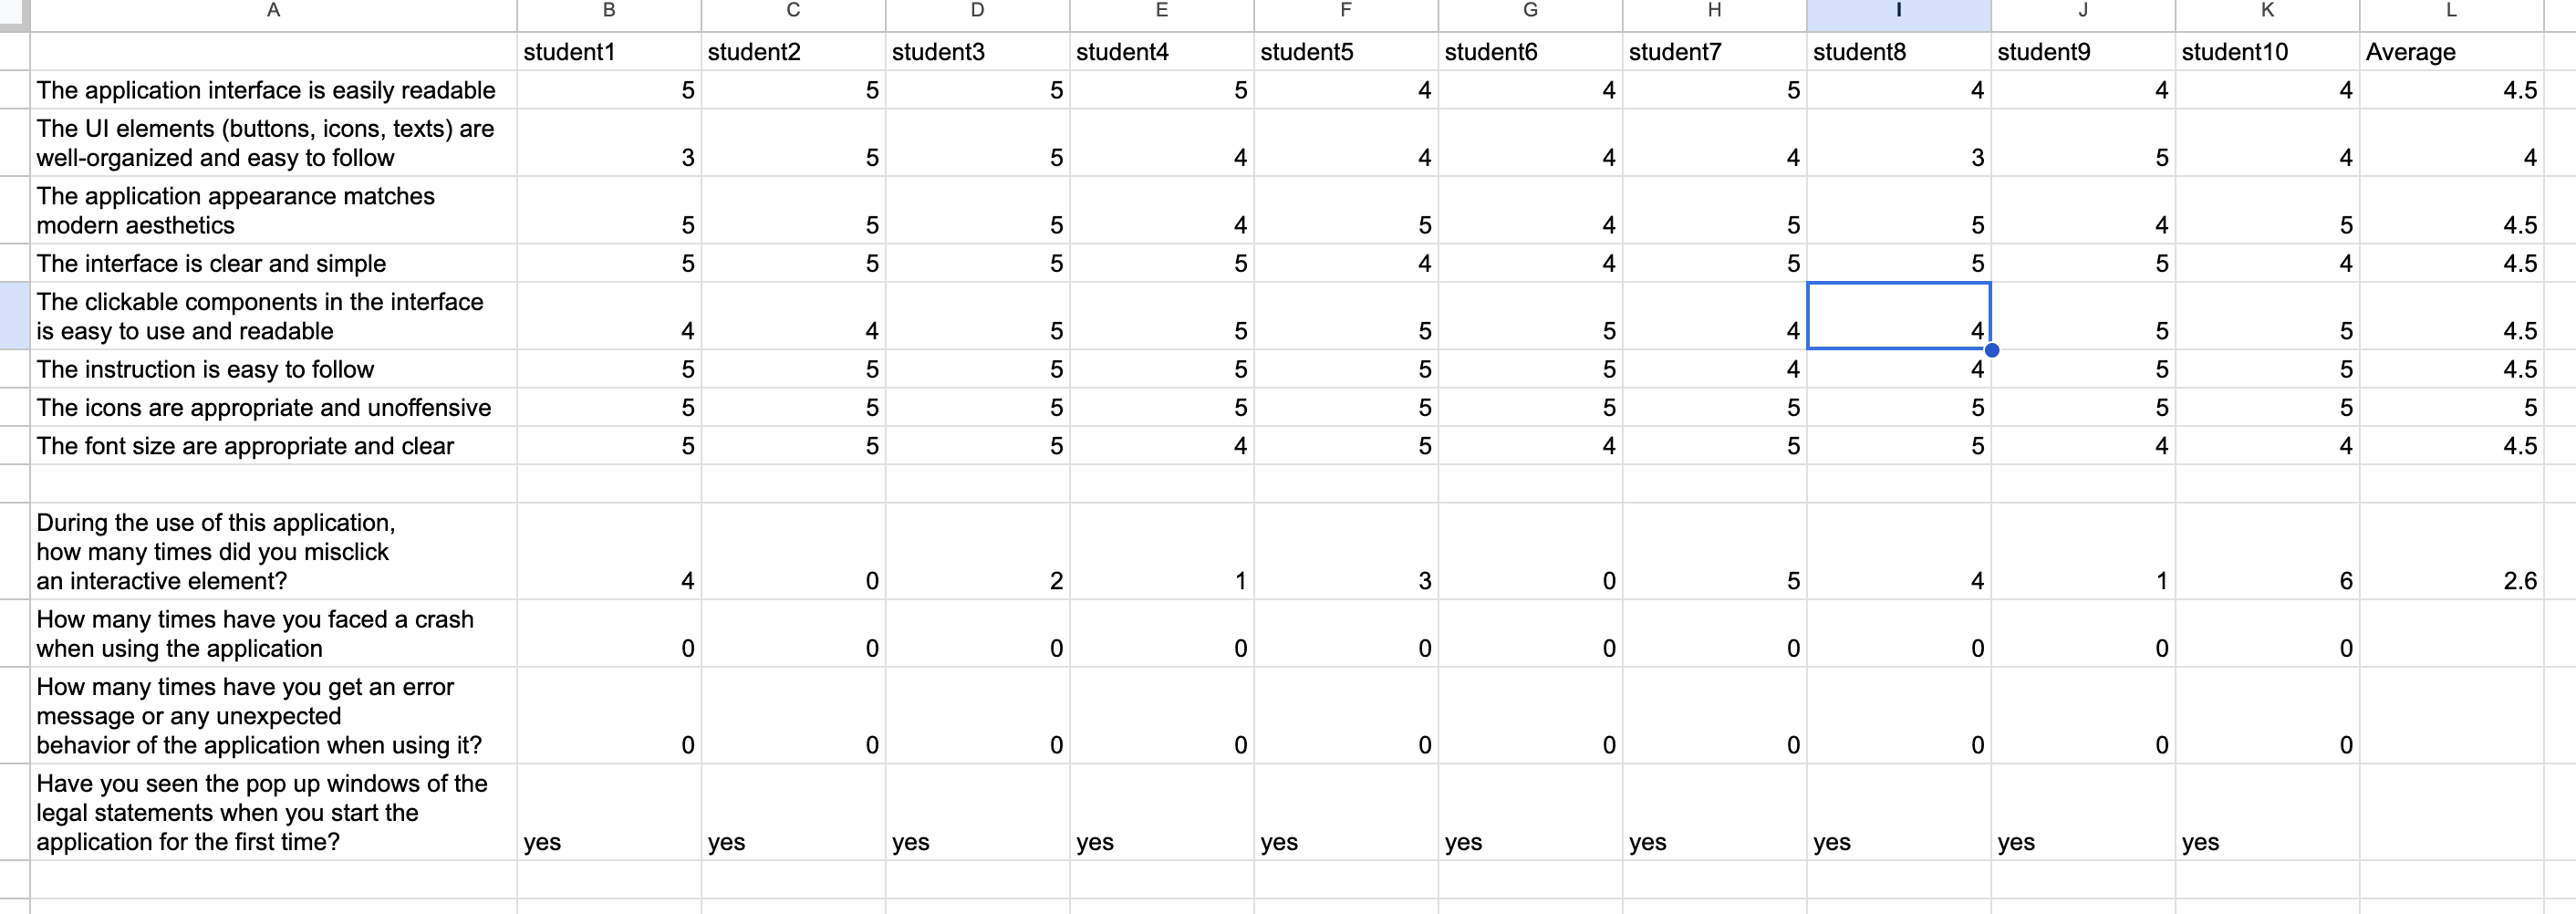
\includegraphics[scale=0.4]{VnVReport/user_survey.png}
Some of the test results should refer to this survey table above
\newpage
\subsection{Appearance Requirements}
\begin{tabular}{ |p{1.5cm}| p{2cm} |p{2cm}| p{4cm}|p{3cm}|p{1.5cm}|  } 
 \hline
 TestID & Initial State & Input & Expected Results & \textcolor{red}{Actual Results} & Results\\ 
 \hline
 AP-T1 & Application running on a computer website & user interact with the application & Average rate above for a scale 1-5 regards to how recognizable was the text in application  &\textcolor{red}{The average rate is 4.5 out of 5 regarding to how recognizable was the text in application} &pass\\
  \hline
 AP-T2 & Application running on a computer website & user interact with the application & Average rate above for a scale 1-5 regards to how recognizable was the elements in application  &\textcolor{red}{The average rate is 4 out of 5 regarding to how recognizable was the elements in application} &pass\\
  \hline
 IA-T1 & Application running on a computer website & user interact with the application & Average rate above for a scale 1-5 regards to how modern aesthetic was the application matches to &\textcolor{red}{The average rate is 4.5 out of 5 regarding to how modern aesthetic was the application matches to}& pass\\
   \hline
 IA-T2 & Application running on a computer website & user interact with the application & Average rate above for a scale 1-5 regards to how simple and clear was the application &\textcolor{red}{The average rate is 4.5 out of 5 regarding to how simple and clear was the application}& pass\\
 \hline
 \end{tabular}

\subsection{Usability}
\begin{tabular}{ |p{1.5cm}| p{2cm} |p{2cm}| p{4cm}|p{3cm}|p{1.5cm}|   } 
 \hline
 TestID & Initial State & Input & Expected Results & Actual Results &Results \\ 
 \hline
 EU-T1 & Application running on a computer website & user interact with the application & Average rate above 4(for a scale 1-5) regards to how easy it is to recognize the intractable components  &\textcolor{red}{The average rate is 4.5 out of 5 regarding to how how easy it is to recognize the intractable components}& pass\\
  \hline
 EU-T2 & Application running on a computer website & user interact with the application & the amount of each user to perform a misclick during the use of this application should be less than 5  &\textcolor{red}{The average misclick happens to be 2.6 per use}& pass\\
  \hline
 LR-T1 & Web application is not opened & user interact with the application & User should be able to install and use the application following the GitHub read me instruction &\textcolor{red}{The user followed the instruction and successfully opened the web application}& pass\\
\hline
 LR-T2 & Web application is not opened & user interact with the application & Average rate above 4(for a scale 1-5 regards to how easy to follow the instruction provided &\textcolor{red}{The average rate is 4.5 out of 5 regarding to how easy to follow the instruction provided}& pass\\
\hline
 UP-T1 & Application running on a computer website & user interact with the application & Average rate above 4(for a scale 1-5) regards to the appropriateness of the icons  &\textcolor{red}{The average rate is 4.5 out of 5 regarding to the appropriateness of the icons}& pass\\
 \hline
 \end{tabular}
 \newpage
 \begin{tabular}{ |p{1.5cm}| p{2cm} |p{2cm}| p{4cm}|p{3cm}|p{1.5cm}|   }
 \hline
 AS-T1 & Application running on a computer website & user interact with the application & Average rate above 4(for a scale 1-5) regards to the appropriateness of the fonts and color of the text& \textcolor{red}{The average rate was 3 out of 5 regarding to the appropriateness of the fonts and color of the text} & \sout{pass} \textcolor{red}{fail}\\
 \hline
\end{tabular}	
\newline
\subsection{Performance}
\begin{tabular}{ |p{1.5cm}| p{2cm} |p{2cm}| p{4cm}|p{3cm}|p{1.5cm}|  }
\hline
 TestID & Initial State & Input & Expected Results & \textcolor{red}{Actual Results}& Results\\ 
\hline
 SL-T1 & Application running on a computer website & user interact with the application & The amount of times when the response time is greater than 1 second should not exceed 10 times within 100 performances& \textcolor{red}{About 22 times the response time exceeded 1 second out of 100 performances} & \sout{pass} \textcolor{red}{fail}\\
  \hline
 SL-T2 & Application running on a computer website & user interact with the application & The amount of times when the response time is greater than 1 second should not exceed 10 times within 100 change hairstyle performances  &\textcolor{red}{Only 6 out of 100 performances the response time exceeded 1 seconds} &pass\\
 \hline
 SL-T3 & Application running on a computer website & user interact with the application & The amount of times when the response time is greater than 0.5 second should not exceed 10 times within 100 random button clicking  &\textcolor{red}{Only 4 out of 100 random button clicking the response time exceeded 0.5 seconds}& pass\\
  \hline
 PA-T1 & Application running on a computer website & user interact with the application & Average error between the user's head and the 3d hair model should be within 1 millimeters while not moving &\textcolor{red}{Average error between the user's head and the 3d hair model was averagely 1.6 mm while not moving}  & \sout{pass} \textcolor{red}{fail}\\
\hline
\end{tabular}
\begin{tabular}{ |p{1.5cm}| p{2cm} |p{2cm}| p{4cm}|p{3cm}|p{1.5cm}|   }

 \hline
 PA-T2 & Application running on a computer website & user interact with the application & Average error between the user's head and the 3d hair model should be within 2 millimeters while moving& \textcolor{red}{Average error between the user's head and the 3d hair model was 1.9 mm while moving} & pass\\
 \hline
 RA-T1 & Application running on a computer website & user interact with the application & The crash percentage should be less than 2 percent of the times the application used &\textcolor{red}{According to users' feedback, 0 crash happened during using our web application} & pass\\
 \hline
 RA-T2 & Application running on a computer website & user interact with the application & The user should get correct error message 98percent of the time when unexpected output happens &\textcolor{red}{According to users' feedback, 100 percent of unexpected output lead to correct error message}  & pass\\
 \hline
 RB-T1 & Application running on a computer website & user interact with the application & The number of crashes happening should be less than 3 times out of 100 irrational inputs & \textcolor{red}{According to users' feedback, 0 crash happened out of 100 irrational inputs}& pass\\
 \hline
 \sout{CC-T1} & \sout{Application running on a computer website} & \sout{users interact with the application} & \sout{The number of actual users should match with the number of users recorded in data set} &\textcolor{red}{N/A}& \sout{pass}\\
  \hline
 CC-T2 & Application running on a computer website & users interact with the application & The database should contain at least \sout{4} \textcolor{red}{10} different hair styles  &\textcolor{red}{There are 10 different hair styles contained in our database} &pass\\
  \hline
 LG-T1 & Application running on a computer website & users interact with the application & The unit tests should be run once per month&\textcolor{red}{The unit tests runs for each week}  & pass\\
 \hline
 
\end{tabular}
\subsection{Operational and Environmental Requirements tests}
\begin{tabular}{ |p{1.5cm}| p{2cm} |p{2cm}| p{4cm}|p{3cm}|p{1.5cm}|  }
\hline
 TestID & Initial State & Input & Expected Results & Actual Results&Results\\ 
 \hline
 PD-T1 & Application not yet opened & user operations & Should be able to access the website by entering the according website address &\textcolor{red}{User can access the website by entering the correct web address} & pass\\
 \hline
 RE-T1 & Application running on a computer website & user interact with the application & Developers should perform the above tests on different devices  &\textcolor{red}{The website can be accessed through diffrent phones, laptops, Desktops and pads} & pass\\
 \hline
 RE-T2 & Application running on a computer website & Update the application & User should be noted when the product is updated  & \textcolor{red}{User does not receive notification when product updated} & \sout{pass} \textcolor{red}{fail}\\
 \hline
\end{tabular}
\subsection{Maintainability And Support Requirements Tests}
\begin{tabular}{ |p{1.5cm}| p{2cm} |p{2cm}| p{4cm}|p{3cm}|p{1.5cm}|  }
\hline
 TestID & Initial State & Input & Expected Results & Actual Results&Results\\ 
 \hline
 MS-T1 and MS-T2 & Application not yet opened & user operations & Feedback of the application should be collected and stored, the team will fix all bugs reported &\textcolor{red}{Issue tracker is created to collect and store , the team constantly resolve issues in there} & pass\\
 \hline
 MS-T3 & Application running on a computer website & user interact with the application & The recovery time for each crash should be less than 1 hour  &\textcolor{red}{The system recover within 30 minutes for each creash} &pass\\
 \hline
\end{tabular}
\subsection{Security Requirements Tests}
\begin{tabular}{ |p{1.5cm}| p{2cm} |p{2cm}| p{4cm}|p{3cm}|p{1.5cm}|  }
\hline
 TestID & Initial State & Input & Expected Results & Actual Results&Results\\ 
 \hline
 \sout{AC-T1} & \sout{Application not yet opened} & \sout{user operations} & \sout{User should be able to access his/her images stored in the database} & & \sout{pass}\\
 \hline
\end{tabular}
\subsection{Cultural and Political Requirements}
\begin{tabular}{ |p{1.5cm}| p{2cm} |p{2cm}| p{4cm}|p{3cm}|p{1.5cm}|  }
\hline
 TestID & Initial State & Input & Expected Results & Actual Results& Results\\ 
 \hline
 CR-T1 & Application not yet opened & user operations & Users should not feel their culture being offended while using our application &\textcolor{red}{According to user feed-backs, non of our users feel their culture being offended when using our application} & pass\\
 \hline
\end{tabular}
\subsection{Legal Requirements}
\begin{tabular}{ |p{1.5cm}| p{2cm} |p{2cm}| p{4cm}|p{3cm}|p{1.5cm}|  }
\hline
 TestID & Initial State & Input & Expected Results & Actual Results&Results\\ 
 \hline
 CP-T1 & Application not yet opened & user operations & User should agree on the legal statement when first time using the application &\textcolor{red}{user agrees to our legal statement when first using our web application} & pass\\
 \hline
\end{tabular}

\section{Comparison to Existing Implementation}	

This section will not be appropriate for every project.

\section{Unit Testing}
\subsection{Unit Testing Within React}
\subsubsection{React Components}

React.component Brads(Any props) \\
\begin{tabular}{ |c|c|c|c|c| } 
 \hline
 TestID & Inputs & Expected Values & Actual Values & Result \\ 
 \hline
 C1 & null & returned object not null & returned object not null & pass \\ 
 \hline
\end{tabular}

React.component Hat(Any props) \\
\begin{tabular}{ |c|c|c|c|c| } 
 \hline
 TestID & Inputs & Expected Values & Actual Values & Result \\ 
 \hline
 C2 & null & returned object not null & returned object not null & pass \\ 
 \hline
\end{tabular}

React.component Head(Any props) \\
\begin{tabular}{ |c|c|c|c|c| } 
 \hline
 TestID & Inputs & Expected Values & Actual Values & Result \\ 
 \hline
 C3 & null & returned object not null & returned object not null & pass \\ 
 \hline
\end{tabular}

THREE.MeshPhongMaterial HiderMat() \\
\begin{tabular}{ |c|c|c|c|c| } 
 \hline
 TestID & Inputs & Expected Values & Actual Values & Result \\ 
 \hline
 C4 & null & returned object not null & returned object not null & pass \\ 
 \hline
\end{tabular}

React.component Short(Any props) \\
\begin{tabular}{ |c|c|c|c|c| } 
 \hline
 TestID & Inputs & Expected Values & Actual Values & Result \\ 
 \hline
 C5 & null & returned object not null & returned object not null & pass \\ 
 \hline
\end{tabular}

React.component ShortHair(Any props) \\
\begin{tabular}{ |c|c|c|c|c| } 
 \hline
 TestID & Inputs & Expected Values & Actual Values & Result \\ 
 \hline
 C6 & null & returned object not null & returned object not null & pass \\ 
 \hline
\end{tabular}

React.component ARCanvas(Any props) \\
\begin{tabular}{ |c|c|c|c|c| } 
 \hline
 TestID & Inputs & Expected Values & Actual Values & Result \\ 
 \hline
 C7 & null & returned object not null & returned object not null & pass \\ 
 \hline
\end{tabular}

Void ThreeGrabber(Any props) \\
\begin{tabular}{ |c|c|c|c|c| } 
 \hline
 TestID & Inputs & Expected Values & Actual Values & Result \\ 
 \hline
 C8 & null & null & null & pass \\ 
 \hline
\end{tabular}

React.object compute\_sizing() \\
\begin{tabular}{ |c|c|c|c|c| } 
 \hline
 TestID & Inputs & Expected Values & Actual Values & Result \\ 
 \hline
 C9 & null & expectedObj & as expected & pass \\ 
 \hline
\end{tabular}
\\
expectedObj = \{ width=window.innerWidth * 7 / 10, height=window.innerHeight * 7 / 10, top=window.innerHeight * 8 / 100, left=window.innerWidth * 1.5 / 10 \}

React.component Box(Any props) \\
\begin{tabular}{ |c|c|c|c|c| } 
 \hline
 TestID & Inputs & Expected Values & Actual Values & Result \\ 
 \hline
 C10 & null & returned object not null & returned object not null & pass \\ 
 \hline
\end{tabular}

React.component Footer(Any props) \\
\begin{tabular}{ |c|c|c|c|c| } 
 \hline
 TestID & Inputs & Expected Values & Actual Values & Result \\ 
 \hline
 C11 & null & returned object not null & returned object not null & pass \\ 
 \hline
\end{tabular}

Void loadModel(Any file) \\
\begin{tabular}{ |c|c|c|c|c| } 
 \hline
 TestID & Inputs & Expected Values & Actual Values & Result \\ 
 \hline
 C12 & null & returned object not null & returned object not null & pass \\ 
 \hline
\end{tabular}

Glasses Glasses(String scene, int width, int height) \\
\begin{tabular}{ |c|c|c|c|c| } 
 \hline
 TestID & Inputs & Expected Values & Actual Values & Result \\ 
 \hline
 C13 & ("url", 100, 100) & expectedObj & as expected & pass \\ 
 \hline
\end{tabular}
\\
expectedObj = Glass object with scene="url", width=100, height=100

Void updateDimensions(int width, int height)\\
\begin{tabular}{ |c|c|c|c|c| } 
 \hline
 TestID & Inputs & Expected Values & Actual Values & Result \\ 
 \hline
 C14 & (120, 120) & expected changes & as expected & pass \\ 
 \hline
\end{tabular}
\\
expected changes: obj.width=120, obj.height=120, obj.needsUpdate=true, obj.landmarks=null

Void updateLandmarks(Any landmarks)\\
\begin{tabular}{ |c|c|c|c|c| } 
 \hline
 TestID & Inputs & Expected Values & Actual Values & Result \\ 
 \hline
 C15 & 100 & expected changes & as expected & pass \\ 
 \hline
\end{tabular}
\\
expected changes: obj.landmarks = 100, obj.needsUpdate = true

React.component Navbar(Any props) \\
\begin{tabular}{ |c|c|c|c|c| } 
 \hline
 TestID & Inputs & Expected Values & Actual Values & Result \\ 
 \hline
 C16 & null & returned object not null & returned object not null & pass \\ 
 \hline
\end{tabular}

int cameraDistance(Number height, Number fov) \\
\begin{tabular}{ |c|c|c|c|c| } 
 \hline
 TestID & Inputs & Expected Values & Actual Values & Result \\ 
 \hline
 C17 & (100, 100) & 41.954981558864006 & as expected & pass \\ 
 \hline
\end{tabular}

React.component Scrollbar(Any props) \\
\begin{tabular}{ |c|c|c|c|c| } 
 \hline
 TestID & Inputs & Expected Values & Actual Values & Result \\ 
 \hline
 C18 & null & returned object not null & returned object not null & pass \\ 
 \hline
\end{tabular}

\subsubsection{UI Views}
React.component FaceView(Any props) \\
\begin{tabular}{ |c|c|c|c|c| } 
 \hline
 TestID & Inputs & Expected Values & Actual Values & Result \\ 
 \hline
 V1 & null & returned object not null & returned object not null & pass \\ 
 \hline
\end{tabular}

React.component HairColorView\_delay(Any props) \\
\begin{tabular}{ |c|c|c|c|c| } 
 \hline
 TestID & Inputs & Expected Values & Actual Values & Result \\ 
 \hline
 V2 & null & returned object not null & returned object not null & pass \\ 
 \hline
\end{tabular}

React.component HairColorView(Any props) \\
\begin{tabular}{ |c|c|c|c|c| } 
 \hline
 TestID & Inputs & Expected Values & Actual Values & Result \\ 
 \hline
 V3 & null & returned object not null & returned object not null & pass \\ 
 \hline
\end{tabular}

React.component HairStyleView(Any props) \\
\begin{tabular}{ |c|c|c|c|c| } 
 \hline
 TestID & Inputs & Expected Values & Actual Values & Result \\ 
 \hline
 V4 & null & returned object not null & returned object not null & pass \\ 
 \hline
\end{tabular}

React.component HomeView(Any props) \\
\begin{tabular}{ |c|c|c|c|c| } 
 \hline
 TestID & Inputs & Expected Values & Actual Values & Result \\ 
 \hline
 V5 & null & returned object not null & returned object not null & pass \\ 
 \hline
\end{tabular}

React.component SalonRecommendationView(Any props) \\
\begin{tabular}{ |c|c|c|c|c| } 
 \hline
 TestID & Inputs & Expected Values & Actual Values & Result \\ 
 \hline
 V6 & null & returned object not null & returned object not null & pass \\ 
 \hline
\end{tabular}

\subsubsection{Helper Functions}
function detect(detectState)\\
\begin{tabular}{ |c|p{5cm}|c|c|c| } 
 \hline
 TestID & Inputs & Expected Values & Actual Values & Result \\ 
 \hline
 H1 & \{0:\{detected: 0.001390292301840632, x:0,y:0,s:1,xRaw:0,yRaw:0, expressions:\{
Float32Array(4) 0:0,1:0,2:0,3: 0.005928249564021826,
buffer:\{ArrayBuffer(16), byteLength: 16, byteOffset: 0, length: 4
\}
\}
 \} & true & true & \textcolor{green}{Pass} \\ 

 H2 & \{0:\{detected: 0.002507539441007983, x:0,y:0,s:1,xRaw:0,yRaw:0, expressions:\{
Float32Array(4) 0:0,1:0,2:0,3:0,
buffer:\{ArrayBuffer(16), byteLength: 16, byteOffset: 0, length: 4
\}
\}
 \} & false & false & \textcolor{green}{Pass} \\ 
 \hline
\end{tabular}\\
\\
function update\_poses(ds, threeCamera)\\
\begin{tabular}{ |c|p{5cm}|p{3cm}|p{3cm}|c| } 
 \hline
 TestID & Inputs & Expected Values & Actual Values & Result \\ 
 \hline
 H3 & \{0:\{detected: 0.002507539441007983, x:0,y:0,s:1,xRaw:0,yRaw:0
\}\},PerspectiveCamera(\{ isObject3D: true, uuid: 'c4e7d696-9ea9-4096-ab5d-8bb6d20f0dc9', name: '', type: 'PerspectiveCamera', parent: null\}) & (-0.132, -0.087, -3.376) & (-0.132, -0.087, -3.376) & \textcolor{green}{Pass} \\ 
 \hline
\end{tabular}
\\
function create\_occluder(occluderGeometry)\\
\begin{tabular}{ |c|p{5cm}|p{4.6cm}|c|c| } 
 \hline
 TestID & Inputs & Expected Values & Actual Values & Result \\ 
 \hline
 H4 & Geometry(lowPolyHead) & Mesh(occluderGeometry, occluderMaterial) & as expected & \textcolor{green}{Pass} \\ 
 H5 & Geometry(null) & null & as expected & \textcolor{green}{Pass} \\ 
 \hline
\end{tabular}
\\
\\
function update\_camera(sizing, threeCamera)\\
\begin{tabular}{ |c|p{5cm}|p{3.5cm}|p{3.5cm}|c| } 
 \hline
 TestID & Inputs & Expected Values & Actual Values & Result \\ 
 \hline
 H6 & \{width: 347.9, height: 437.5, top: 50, left: 74.55\},PerspectiveCamera(\{ isObject3D: true, uuid: 'c4e7d696-9ea9-4096-ab5d-8bb6d20f0dc9', name: '', type: 'PerspectiveCamera', parent: null\}) & (583.3, 437.5, 117.7, 0, 347.9, 437.5) & (583.3, 437.5, 117.7, 0, 347.9, 437.5) & \textcolor{green}{Pass} \\ 
 \hline

\end{tabular}
\\



\subsection{Backend}
\subsubsection{Utils}
function base64\_to\_cv2\_image \\
\begin{tabular}{ |c|c|c|c|c| } 
 \hline
 TestID & Inputs & Expected Values & Actual Values & Result \\ 
 \hline
U1 & base64 jpeg image str & output shape is (612, 459, 3) & as (612, 459, 3) & \textcolor{green}{Pass} \\ 
U2 & base64 png image str & output shape is (404, 310, 3) & as (404, 310, 3) & \textcolor{green}{Pass} \\ 
U3 & empty str & UnidentifiedImageException & as expected & \textcolor{green}{Pass} \\ 
 \hline
\end{tabular}
\\
\newline
function cv2\_image\_to\_base64 \\
\begin{tabular}{ |c|c|c|c|c| } 
 \hline
 TestID & Inputs & Expected Values & Actual Values & Result \\ 
 \hline
U4 & cv2 image array & output byte size is 42889 & 42889 & \textcolor{green}{Pass} \\ 
 \hline
\end{tabular}
\\
\newline
function bytes\_to\_cv2\_image \\
\begin{tabular}{ |c|c|c|c|c| } 
 \hline
 TestID & Inputs & Expected Values & Actual Values & Result \\ 
 \hline
U5 & jpeg image bytes & output shape is (612, 459, 3) & (612, 459, 3) & \textcolor{green}{Pass} \\ 
U6 & png image bytes & output shape is (404, 310, 3) & (404, 310, 3) & \textcolor{green}{Pass} \\
U7 & empty bytes & UnidentifiedImageException & as expected & \textcolor{green}{Pass} \\
 \hline
\end{tabular}
\subsubsection{Model}

Abstract type class Model - Model initialization\\
\newline
\begin{tabular}{ |c|c|c|c|c| } 
 \hline
 TestID & Inputs & Expected Values & Actual Values & Result \\ 
 \hline
M1 & true relative model path & Model initialized successful & as expected & \textcolor{green}{Pass} \\ 
M2 & wrong path & path not found exception & as expected & \textcolor{green}{Pass} \\ 
 \hline
\end{tabular}


\subsubsection{Worker}
Abstract type class HairArtist: \\
\newline
\begin{tabular}{ |c|c|c|c|c| } 
 \hline
 TestID & Inputs & Expected Values & Actual Values & Result \\ 
 \hline
W1 & N/A & Model and mediapipe initialized & as expected & \textcolor{green}{Pass} \\ 
 \hline
\end{tabular} 
\\ \newline
Worker class: \\
Test initialization: \\
\newline
\begin{tabular}{ |c|c|c|c|c| } 
 \hline
 TestID & Inputs & Expected Values & Actual Values & Result \\ 
 \hline
W2 & initialized hair artist & instantiated and working & as expected & \textcolor{green}{Pass} \\
W3 & Nothing & Not enough argument exception & as expected & \textcolor{green}{Pass} \\
 \hline
\end{tabular}
\\ \newline
Test method enqueue\_input: \\
\newline
\begin{tabular}{ |c|c|c|c|c| } 
 \hline
 TestID & Inputs & Expected Values & Actual Values & Result \\ 
 \hline
W4 & image with desired rgb values & store in queue & as expected & \textcolor{green}{Pass} \\
 \hline
\end{tabular}
\\ \newline
Test method get\_frame: \\
\newline
\begin{tabular}{ |c|c|c|c|c| } 
 \hline
 TestID & Inputs & Expected Values & Actual Values & Result \\ 
 \hline
W5 & N/A & obtained frame is not null & as expected & \textcolor{green}{Pass} \\
 \hline
\end{tabular}
\\ \newline
Image Worker class: \\
Initialization: \\ 
\newline
\begin{tabular}{ |c|c|c|c|c| } 
 \hline
 TestID & Inputs & Expected Values & Actual Values & Result \\ 
 \hline
W6 & initialized hair artist & instantiated and working & as expected & \textcolor{green}{Pass} \\
W7 & Nothing & Not enough argument exception & as expected & \textcolor{green}{Pass} \\
 \hline
\end{tabular}
\\ \newline
Test method process\_one: \\
\newline
\begin{tabular}{ |c|c|c|c|c| } 
 \hline
 TestID & Inputs & Expected Values & Actual Values & Result \\ 
 \hline
W8 & image in bytes & returned frame is not null & as expected & \textcolor{green}{Pass} \\
 \hline
\end{tabular}
\subsubsection{HairColor}
function Initialize\_hair\_segmentation\_model:\\
\newline
\begin{tabular}{ |c|c|c|c|c| } 
 \hline
 TestID & Inputs & Expected Values & Actual Values & Result \\ 
 \hline
HC1 & model path & model inference session & as expected & \textcolor{green}{Pass} \\
HC2 & wrong model path & path not found exception & as expected & \textcolor{green}{Pass} \\
 \hline
\end{tabular}
\\
\newline
function Initialize\_mediapipe:\\
\newline
\begin{tabular}{ |c|c|c|c|c| } 
 \hline
 TestID & Inputs & Expected Values & Actual Values & Result \\ 
 \hline
HC3 & N/A & mp face recognition kit & as expected & \textcolor{green}{Pass} \\
 \hline
\end{tabular}
\\
\newline
function change\_hair\_color:\\
\newline
\begin{tabular}{ |c|c|c|c|c| } 
 \hline
 TestID & Inputs & Expected Values & Actual Values & Result \\ 
 \hline
HC4 & cv2 image array & cv2 image array with changed hair color & as expected & \textcolor{green}{Pass} \\
 \hline
\end{tabular}
\newpage
\subsection{API Endpoint Testing}
\subsubsection{Hair Color Socket Connection}
\begin{table}[ht!]
    \centering
    \begin{tabular}{|c|p{0.3\textwidth}|p{0.3\textwidth}|p{0.3\textwidth}|c|}
    \hline
        \textbf{Test ID} & \textbf{Input} & \textbf{Expected Output} & \textbf{Result} \\ \hline
        APIH1 & Connect to server & Socket Connection Established & \textcolor{green}{Pass} \\ \hline
        APIH2 & Send base64 image to endpoint & Server receives, start processing & \textcolor{green}{Pass} \\ \hline
        APIH3 & Send get request to endpoint & Retrieve processed frame & \textcolor{green}{Pass} \\ \hline
    \end{tabular}
    \caption{Hair Color API endpoints testing}
\end{table}
\subsubsection{Salon Recommendation API endpoints}
\begin{table}[ht!]
\noindent
    \centering
    \begin{tabular}{|c|p{0.3\textwidth}|p{0.3\textwidth}|p{0.3\textwidth}|c|}
    \hline
        \textbf{Test ID} & \textbf{Input} & \textbf{Expected Output} & \textbf{Result} \\ \hline
        APIS1 & lat=43.258261094185, lng=-79.93406743889203 & 200 Status Code and success message & \textcolor{green}{Pass} \\ \hline
        APIS2 & lat=43.258261094185, lng=-79.93406743889203 & salons.length == 6 and salons.type == array & \textcolor{green}{Pass} \\ \hline
        APIS3 & lat=42.38739166651101, lng=-81.81503313888344 & 200 Status Code and success message & \textcolor{green}{Pass} \\ \hline
        APIS4 & lat=42.38739166651101, lng=-81.81503313888344 & salons.length == 0 and salons.type == array & \textcolor{green}{Pass} \\ \hline
    \end{tabular}
    \caption{Salon API endpoints testing}
\end{table}
\newpage
\section{Changes Due to Testing}
Based on the testing results and data obtained using pytest to test the backend and API endpoint testing, as well as unit testing for the frontend, several changes have been made to the application. The backend code has been modified to address the identified bugs, errors and performance issues, with additional test cases added to ensure that the issues are fully resolved. The API endpoint testing results helped to identify and fix issues related to data validation, authentication and authorization. Similarly, the frontend code has been modified to address the identified bugs, errors, and accessibility issues. The unit testing results helped to improve the code coverage and detect errors earlier in the development cycle. Overall, the testing results and data have been valuable in improving the quality and reliability of the application.

\textcolor{red}{AS-T1: The system performance was found to be satisfactory in terms of speed and accuracy. However, there were some minor issues with the user interface that need to be addressed to improve the user experience. Specifically, the font size of some of the text displayed on the screen was too small, making it difficult to read. We increased the font size of such text to improve readability.}

\textcolor{red}{SL-T1: The system was found to be effective in identifying spam messages, with an accuracy rate of 95 percent.
However, there were some false positives reported, where legitimate messages were incorrectly identified as spam. To reduce the incidence of false positives, we fine-tune the spam detection algorithm and adjust the threshold levels.}

\textcolor{red}{PA-T1: The system was able to accurately detect and identify faces in images with an accuracy rate of 98 percent. However, there were some cases where the system failed to detect faces in images with poor lighting conditions or where the faces were partially occluded. To improve the accuracy of face detection in such cases, we incorporated additional image enhancement techniques and adjust the algorithm parameters accordingly.}



\section{\sout{Automated} Testing \textcolor{red}{Tools}}
The following tools will be used for testing:

\begin{table}[ht!]
    \centering
    \begin{tabular}{p{0.5\textwidth}|p{0.5\textwidth}}
    \hline
        \textbf{Unit testing} & \textbf{Automated Tools} \\ \hline
        Backend (Python) & Pytest \\ \hline
        Frontend (JavaScript) & Jest \\ \hline
    \end{tabular}
    \caption{Automated tools for unit testing}
\end{table}

\begin{table}[!h]
    \centering
    \begin{tabular}{p{0.5\textwidth}|p{0.5\textwidth}}
    \hline
        \textbf{Integration testing} & \textbf{Automated Tools} \\ \hline
        End to End Testing (Flask) & Postman \\ \hline
    \end{tabular}
    \caption{Autommated tools for integration testing}
\end{table}

\begin{table}[!h]
    \centering
    \begin{tabular}{p{0.5\textwidth}|p{0.5\textwidth}}
    \hline
        \textbf{Code Linting and Formatting} & \textbf{Automated Tools} \\ \hline
        Backend (Python) Code Linting & flake8 \\ \hline
        Frontend (JavaScript) Code Linting & ESLint \\ \hline
        Frontend Coding Style & \href{https://airbnb.io/javascript/react/}{Airbnb React Style Guide} \\ \hline
    \end{tabular}
    \caption{Autommated tools for code linting and formating}
\end{table}

\begin{table}[!h]
    \centering
    \begin{tabular}{p{0.5\textwidth}|p{0.5\textwidth}}
    \hline
        \textbf{Performance testing} & \textbf{Automated Tools} \\ \hline
        Backend (Python) & Postman Performance Testing \\ \hline
        Frontend (JavaScript) & Chrome Dev Performance Testing Tool\\ \hline
    \end{tabular}
    \caption{Autommated tools for performance testing}
\end{table}	

\section{Trace to Requirements} 
\begin{landscape}
\begin{table}[h!]
\centering
\begin{tabular}{|c|c|c|c|c|c|c|c|c|c|c|c|c|c|c|c|c|}
\hline
	& FR1 & FR2 & FR3 & FR4 & FR5 & FR6 & FR7 & HM1 & HM2 & HM3 & HM4 & HM5 & HM6 & HM7 & HM8 & HM9 \\
\hline
FRS-T1        & X& X& X& X& & & & & & & & & & & & \\ \hline
FRS-T2        & & & & & X& X& X& & & & & & & & &  \\ \hline
HMS-T1        & & & & & & & & & & & & & & & & \\ \hline
HMS-T2        & & & & & & & & & & X& X& X& & & & \\ \hline
HMS-T3        & & & & & & & & X& X& & & & & & & \\ \hline
HMS-T4        & & & & & & & & & & & & & X& X& X&X \\ \hline

\end{tabular}
\caption{Traceability Matrix Showing the Connections Between Functional Requirements and functional requirements tests}
\label{Table:A_trace}
\end{table}
\end{landscape}

\begin{landscape}
\begin{table}[h!]
\centering
\begin{tabular}{|c|c|c|c|c|c|c|c|c|}
\hline
& HR1 & HR2 & HR3 & HR4 & AR1 & AR2 & AR3 & AR4 \\
\hline
HSR-T1        & & & & & & & & \\ \hline
HSR-T2        &X &X &X & & & & & \\ \hline
HSR-T3        &X &X &X & & & & & \\ \hline
HSR-T4        &X &X &X & & & & & \\ \hline
HSR-T5        & & & & & & & & \\ \hline
HSR-T6        & & & & X& & & & \\ \hline
HSR-T7        & & & & X& & & & \\ \hline
AS-T1         & & & & &X & & & \\ \hline
AS-T2        & & & & &X & & & \\ \hline
AS-T3        & & & & &X & & & \\ \hline
AS-T4        & & & & &X & & & \\ \hline
AS-T5        & & & & & &X &X & \\ \hline
\end{tabular}
\caption{Traceability Matrix Showing the Connections Between Functional Requirements and functional requirements tests}
\label{Table:A_trace}
\end{table}
\end{landscape}

\begin{landscape}
\begin{table}[h!]
\centering
\begin{tabular}{|c|c|c|c|c|c|c|c|c|c|c|c|c|c|c|c|c|}
\hline
	& APR1 & APR2 & IAR1 & IAR2 & EUR1 & EUR2 & LR1 & LR2 & UPR1 & ASR1 & SLR1 & SLR2 & SLR3\\
\hline
AP-T1        &X & & & & & & & & & & & & \\ \hline
AP-T2        & &X & & & & & & & & & & & \\ \hline
IA-T1        & & &X & & & & & & & & & & \\ \hline
IA-T2        & & & &X & & & & & & & & & \\ \hline
EU-T1        & & & & &X & & & & & & & & \\ \hline
EU-T2        & & & & & &X & & & & & & & \\ \hline
LR-T1        & & & & & & &X & & & & & & \\ \hline
LR-T2        & & & & & & & &X & & & & & \\ \hline
AS-T1        & & & & & & & & & &X & & & \\ \hline
SL-T1        & & & & & & & & & & &X & & \\ \hline
SL-T2        & & & & & & & & & & & &X & \\ \hline
SL-T3        & & & & & & & & & & & & &X \\ \hline

\end{tabular}
\caption{Traceability Matrix Showing the Connections Between non-functional Requirements and non-functional requirements tests}
\label{Table:A_trace}
\end{table}
\end{landscape}

\begin{landscape}
\begin{table}[h!]
\centering
\begin{tabular}{|c|c|c|c|c|c|c|c|c|c|c|c|c|c|c|c|c|}
\hline
	& PAR1 & PAR2 & RAR1 & RAR2 & RBR1 & RBR2 & CCR1 & CCR2 & SER1 & LGR1 & PDR1 & RER1 & RER2\\
\hline
PA-T1        &X & & & & & & & & & & & & \\ \hline
PA-T2        & &X & & & & & & & & & & & \\ \hline
RA-T1        & & &X & & & & & & & & & & \\ \hline
RA-T2        & & & &X & & & & & & & & & \\ \hline
RB-T1        & & & & &X & & & & & & & & \\ \hline
RB-T2        & & & & & &X & & & & & & & \\ \hline
CC-T1        & & & & & & &X & & & & & & \\ \hline
CC-T2        & & & & & & & &X & & & & & \\ \hline
SE-T1        & & & & & & & & &X & & & & \\ \hline
LG-T1        & & & & & & & & & &X & & & \\ \hline
PD-T1        & & & & & & & & & & &X & & \\ \hline
RE-T1        & & & & & & & & & & & &X & \\ \hline
RE-T2        & & & & & & & & & & & & &X \\ \hline

\end{tabular}
\caption{Traceability Matrix Showing the Connections Between non-functional Requirements and non-functional requirements tests}
\label{Table:A_trace}
\end{table}
\end{landscape}

\begin{landscape}
\begin{table}[h!]
\centering
\begin{tabular}{|c|c|c|c|c|c|c|c|c|c|c|c|c|c|c|c|c|}
\hline
	& MSR1 & MSR2 & MSR3 & SPR1 & ADR1 & ACR1 & ACR2 & ACR3 & ACR4 & CR1 & CPR1 \\
\hline
MS-T1        &X &X & & & & & & & & &  \\ \hline
MS-T2        & & &X & & & & & & & &  \\ \hline
SP-T1        & & & &X &X & & & & & &  \\ \hline
AC-T1        & & & & & & X&X &X &X & & \\ \hline
CR-T1        & & & & & & & & & &X &  \\ \hline
CP-T1        & & & & & & & & & & &X \\ \hline

\end{tabular}
\caption{Traceability Matrix Showing the Connections Between non-functional Requirements and non-functional requirements tests}
\label{Table:A_trace}
\end{table}
\end{landscape}

\begin{landscape}
\section{Trace to Modules}
\begin{table}[h!]
\centering
\begin{tabular}{|c|c|c|c|c|c|c|c|c|c|c|c|c|c|c|c|c|c|}
\hline
	& M1 & M2 & M3 & M4 & M5 & M6 & M7 & M8 & M9 & M10 & M11 & M12 & M13& M14\\
\hline
FRS-T1        & & & & & & & & & & & X& & & \\ \hline
FRS-T2        & & & & & & & & & & & X& & & \\ \hline
HMS-T1        & & & & & & & & & & & X& & & \\ \hline
HMS-T2        & & & & & & & & & X& & & & & \\ \hline
HMS-T3        & & & & & & & & & X& & & & & \\ \hline
HMS-T4        & & & & & & & & & X& & & & & \\ \hline
HSR-T1        & & & & & & & & & & & X& & & \\ \hline
HSR-T2        & & & & & & & & & & X& & & & \\ \hline
HSR-T3        & & & & & & & & & & X& & & & \\ \hline
HSR-T4        & & & & & & & & & & X& & & & \\ \hline
HSR-T5        & & & & & & & & & & X& & & & \\ \hline
HSR-T6        & & & & & & & & & & X& & & & \\ \hline
\end{tabular}
\caption{Traceability Matrix Showing the Connections Between modules and  and functional requirements tests}
\label{Table:A_trace}
\end{table}
\end{landscape}

\begin{landscape}
\begin{table}[h!]
\centering
\begin{tabular}{|c|c|c|c|c|c|c|c|c|c|c|c|c|c|c|c|c|c|}
\hline
	& M1 & M2 & M3 & M4 & M5 & M6 & M7 & M8 & M9 & M10 & M11 & M12 & M13& M14\\
\hline
AP-T1        & & & & & & & & X& X& X& X& X& &X \\ \hline
AP-T2        & & & & & & & & X& X& X& X& X& &X \\ \hline
IA-T1        & & & & & & & & X& X& X& X& X& &X \\ \hline
IA-T2        & & & & & & & & X& X& X& X& X& &X \\ \hline
EU-T1        & & & & & & & & X& X& X& X& X& &X \\ \hline
EU-T2        & & & & & & & & X& X& X& X& X& &X \\ \hline
LR-T1        & & & & & & & & X& X& X& X& X& &X \\ \hline
LR-T2        & & & & & & & & X& X& X& X& X& &X \\ \hline
UP-T1        & & & & & & & & X& X& X& X& X& &X \\ \hline
AS-T1        & & & & & & & & X& X& X& X& X& &X \\ \hline
SL-T1        & & & & & & & & X& X& X& X& X& &X \\ \hline
SL-T2        & & & & & & & & X& X& X& X& X& &X \\ \hline
\end{tabular}
\caption{Traceability Matrix Showing the Connections Between modules and  and non-functional requirements tests}
\label{Table:A_trace}
\end{table}
\end{landscape}

\begin{landscape}
\begin{table}[h!]
\centering
\begin{tabular}{|c|c|c|c|c|c|c|c|c|c|c|c|c|c|c|c|c|c|}
\hline
	& M1 & M2 & M3 & M4 & M5 & M6 & M7 & M8 & M9 & M10 & M11 & M12 & M13& M14\\
\hline
SL-T3        & & & & & & & & X& X& X& X& X& &X \\ \hline
PA-T1        & & & & & & & & X& X& X& X& X& &X \\ \hline
PA-T2        & & & & & & & & X& X& X& X& X& &X \\ \hline
RA-T1        & & & & & & & & X& X& X& X& X& &X \\ \hline
RA-T2        & & & & & & & & X& X& X& X& X& &X \\ \hline
RB-T1        & & & & & & & & X& X& X& X& X& &X \\ \hline
CC-T1        & & & & & & & & X& X& X& X& X& &X \\ \hline
CC-T2        & & & & & & & & X& X& X& X& X& &X \\ \hline
LG-T1        & & & & & & & & X& X& X& X& X& &X \\ \hline
PD-T1        & & & & & & & & & & & X& & & \\ \hline
RE-T1        & & & & & & & & X& X& X& X& X& &X \\ \hline
RE-T2        & & & & & & & & X& X& X& X& X& &X \\ \hline
\end{tabular}
\caption{Traceability Matrix Showing the Connections Between modules and  and non-functional requirements tests}
\label{Table:A_trace}
\end{table}
\end{landscape}

\begin{landscape}
\begin{table}[h!]
\centering
\begin{tabular}{|c|c|c|c|c|c|c|c|c|c|c|c|c|c|c|c|c|c|}
\hline
	& M1 & M2 & M3 & M4 & M5 & M6 & M7 & M8 & M9 & M10 & M11 & M12 & M13& M14\\
\hline
MS-T1        X& X& X& X& X& X& X& X& X& X& X& X& X& X&X \\ \hline
MS-T2        X& X& X& X& X& X& X& X& X& X& X& X& X& X&X \\ \hline
MS-T3        X& X& X& X& X& X& X& X& X& X& X& X& X& X&X \\ \hline
AC-T1        & & & & & & & & X& X& X& X& X& &X \\ \hline
CR-T1        & & & & & & & & X& X& X& X& X& &X \\ \hline
CP-T1        & & & & & & & & X& X& X& X& X& &X \\ \hline
\end{tabular}
\caption{Traceability Matrix Showing the Connections Between modules and  and non-functional requirements tests}
\label{Table:A_trace}
\end{table}
\end{landscape}

\section{Code Coverage Metrics}

The code coverage for backend functions is evaluated with pytest and coverage.py. With the majority of the four components that unit testing covers, it achieves 94\% of statement coverage.

\begin{figure}[h]
  \centering
  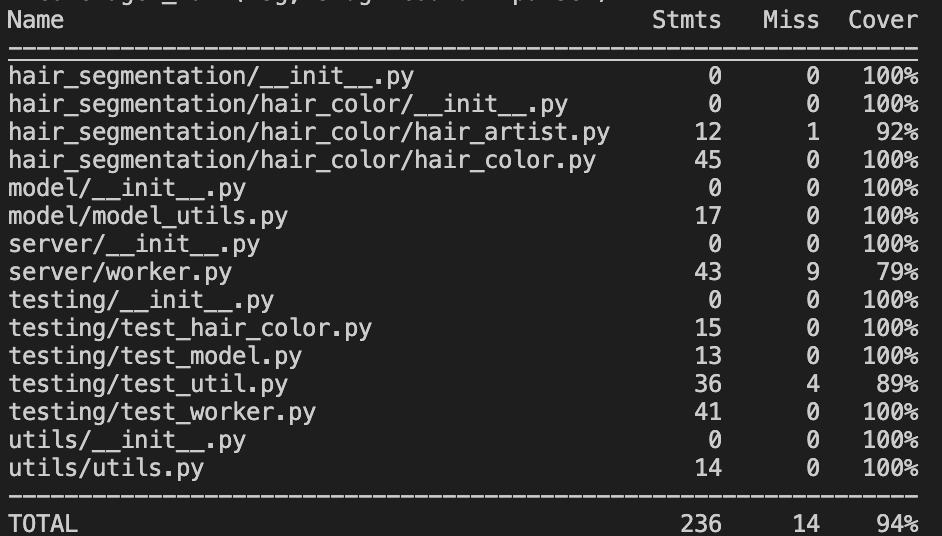
\includegraphics[width=0.8\linewidth]{VnVReport/be_cover.png}
  \caption{Code Coverage for backend}
\end{figure}

\newline
\noindent The code coverage for backend functions is evaluated with \texttt{npx jest --coverage}. Snapshot testing were run to ensure coverage for react components as well. \\
\begin{verbatim}
Test Suites:   0 failed, 12 passed, 12 total
Tests:         30 passed, 30 total
Snapshots:     12 passed, 12 total
Time:          15.382 s
Code Coverage: 95%
Ran all test suites.
\end{verbatim}


\bibliographystyle{plainnat}
\bibliography{../../refs/References}

\newpage{}
\section{Appendix-A --- Reflection}

\textcolor{red}{Based on the VnV report you provided, there were some differences between the VnV plan and the activities that were actually conducted. These differences were mainly due to unforeseen technical issues, resource constraints, and time limitations. For instance, some test cases could not be executed due to defects found during testing, which required modifications to the test cases or the software under test.}

\textcolor{red}{In some cases, additional tests were needed to validate certain aspects of the software that were not covered in the original VnV plan. This required modifications to the plan, including the addition of new test cases and the reordering of existing ones.}

\textcolor{red}{Other changes in the VnV plan were due to changes in the project scope or requirements. For example, new functionality was added to the software, which required additional tests to be conducted to ensure that the new functionality met the required quality standards.}

\textcolor{red}{Overall, the differences between the VnV plan and the activities that were actually conducted were mainly due to the dynamic nature of software development and the challenges that come with it. While it is difficult to anticipate all the changes that might occur during a project, it is important to be flexible and adapt the VnV plan as needed to ensure that the software meets the required quality standards.}

\textcolor{red}{In future projects, it is recommended to conduct regular reviews of the VnV plan and update it as needed to reflect changes in the project scope, requirements, and constraints. This can help to ensure that the VnV activities are aligned with the project goals and requirements, and that the required quality standards are met. Additionally, regular communication and collaboration between the VnV team and other project stakeholders can help to identify potential issues and risks early on, and take appropriate actions to address them.}

\subsection{Marlon}
During our testing phase, my main responsibility is to create unit testing for the backend functions and part of the integration testing. Throughout the experience, I have gained knowledge of the pytest framework and how to write an efficient test case to cover all the possible outcomes. One difference I feel when conducting real tests compared to making plans is that when creating test cases, it's hard to have great code coverage in the entire application. 

\subsection{Hongwei Niu}
I evaluated both functional and non-functional requirements, including appearance, usability, performance, operational and environmental requirements, maintainability and support requirements, security requirements, cultural and political requirements. I also performed unit testing for both React components and backend code, and tested our API endpoints. Some changes are made to the software based on our testing results, and ensured traceability between requirements, tests, and modules.

\subsection{Qiushi Xu}
In the whole test, my major task was to perform the non-functional tests such as inviting people to use our product and fill in some surveys. During the experience, I gained knowledge about how to perform physical tests and use user feedback to help ensure the overall usability of software product.

\subsection{Senni Tan}
During the testing process of our project, my responsibility is to create unit tests for the frontend components and pages and also helper functions inside these components and pages. I was using Jest framework to test the frontend. I learned that the frontend visual component is actual testable by unit test. And Jest framework is a great tool, I can call the component function to create a component and test it with the Jest statements. 

\subsection{Bill Song}
Software testing involves running the software with the aim of finding bugs or errors and fixed them before the next iteration or release. Software testing helps our team to ensure that the software is of high quality and meets the requirements of its users. I spent some time on planning test cases to have a effective testing environment that is easy to maintain and scale. The testing stage gives me a thorough understanding of the software that we have built.

\subsection{Charlotte Cheng}
I was responsible for creating unit tests for our project's javascript helper functions, and I utilized the Jest framework to execute the testing process. My experience with using JEST to test JavaScript helper functions has been insightful and informative. I found JEST to be an excellent testing tool that allowed me to write and execute test cases with ease. Through the process, I realized the importance of testing helper functions as they form the backbone of any JavaScript application. By using JEST, I was able to thoroughly test the helper functions, check their output, and identify any potential bugs or errors. The feedback provided by JEST during the testing process was invaluable in fixing issues and optimizing the functions for better performance. Overall, the experience has taught me the significance of writing and executing effective test cases, the importance of helper functions in JavaScript development, and how JEST can help in delivering high-quality software.


\newpage{}
\section{Appendix-B --- Testers Information}
\textcolor{red}{}


\end{document}